%kelompok 2
%Achmad Fatahillah(1154004)
%Ilga Anne Tri J.S(1154045)
%Maulyanda(1154008)
%Mefi Frinkazela Nikica(1154073)
%Simon Sorba Manangi(1154019)
	
\section{Bangun Ruang}
Bangun ruang merupakan suatu bagian ruang yang dibatasi oleh himpunan titik-titik yang terdapat pada seluruh permukaan bangun tersebut. 
Permukaan bangun tersebut disebut sisi. Bangun ruang memiliki tiga unsur, yaitu 
panjang : merupakan suatu dimensi dalam benda yang menunjukkan sebuah jarak antar ujung satu ke ujung lainnya.
lebar   : merupakan lintasan dalam sebuah bidang.
tinggi  : merupakan ukuran sebuah objek yang diukur secara vertikal.
Bangun ruang memiliki volume. Rumus volume umum pada bangun ruang adalah panjang(p) x lebar(l) x tinggi(t).
Tujuan menghitung volume adalah untuk menghitung berapa banyak ruang yang dapat diisi datau ditempati pada suatu objek.

Sisi bangun ruang adalah suatu himpunan pada titik-titik yang terdapat pada permukaan atau yang membatasi suatu bangun ruang tersebut \cite{umami2013eksperimentasi}

Dalam memilih model untuk permukaan atau sisi, dapat karena kedudukan semua unsur bangun ruang dapat diamati untuk dialihkan dalam gambar\cite{suharjana2008mengenal}. 
Ada beberapa contoh benda yang mewakili gambar bangun ruang\ref{contohbangun}.
\begin{figure}[ht]
    \centerline{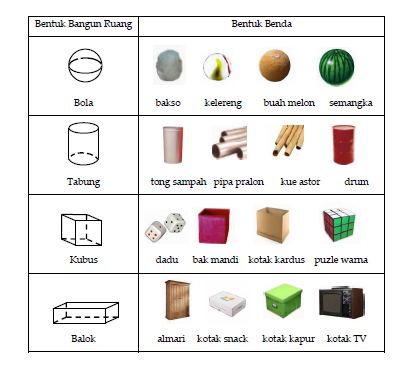
\includegraphics[width=1\textwidth]{figures/contohbangun.png}}
    \caption{beberapa kumpulan gambar yang termasuk dalam bangun ruang}
    \label{contohbangun}
    \end{figure}
 
Bangun ruang sering  disebut bangun 3 dimensi karena memiliki 3 komponen utama sebagai berikut.
1.Sisi  merupakan bidang pada bangun ini memiliki ruang yang membatasi antara bangun ruang dengan ruangansekitarnya 
2.Rusuk merupakan pertemuan antar dua sisi yang berupa ruas garis pada bangun.
3.Titik sudut merupakan titik hasil pertemuan rusuk yang berjumlah tiga atau lebih

Unsur-unsur Bangun Ruang Sisi,rusuk,dantitiksudut. Sebagai mengingatkan bahwa setiap model bangun ruang pasti memiliki sisi, rusuk, dan titiksudut , kecuali bola, tabung,dankerucut.
Bangun ruang, limas, prisma, dan sisi, rusuk, titiksudut serta dikembangkan pada diagonalsisi,diagonalruang, dangaris-garis sejajar.
menggunakan model bangun ruang yang transparan  melihat sisi bangun ruang tersebut, model transparan, bangun ruang dengan model transparan ini juga dapat untuk menggambar bangun ruang, karena semua unsur bangun ruang dapat diamati untuk dialihkan dalam gambar. Setelah mengamati, 
menelusuri, dan memahami unsur-unsur bangun ruang tersebut.

Jenis-Jenis Bangun Ruang yang umum dikenal adalah:
1.  kubus merupakan bangun ruang yang dibatasi oleh enam buah bidang sisi berbentuk persegi dengan ukuran yang sama.
2.balok yaitu bangun ruang dengan dibatasi dengan enam bidang sisi yang memiliki bentuk persegi panjang yang setiap sepasang-sepasang sejajar dan sama ukurannya.
3.prisma yaitu adalah sebuah bangun ruang yang diberikan batas oleh dua buah daerah segitiga yang sejajar sehingga tiga daerah persegi panjang tersebut yang saling berpotongan menurut garis-garis yang sejajar.
4.limas merupakan bangun ruang yang dibatasi leh sebuah daerah segiempat dan empat daerah segitiga yang mempunyai satu titik sudut persekutuan.
5.kerucut merupakan bangun ruang yang dibatasi oleh sebuah bidang lengkung yang simetris terhadap porosnya yang melalui titik pusat lingkaran tersebut.
6.tabung merupakan bangun ruang yang setiap sisinya dibatasin dengan dua bidang lingkaran yang sama-sama sejajar dan sama-sama ukurannya dan satu buah bidang 
     yang memiliki jarak sama jauhnya ke arah poros dan sisi yang simetris ke arah porosnye itu akan memotong dua daerah bidang lingkaran tepat di kedua lingkaran itu .
7.Bola
Jenis-Jenis Bangun Ruang yang umum dikenal adalah dan di dalam kehidupan sehari hari:
1.   Kubus    : dadu, rubik
2.   Balok    : lemari, tv
3.   Prisma    : atap rumah, tenda pramuka
4.   Limas    : piramida, monas
5.   Kerucut: nasi tumppeng yang berbentuk kerucut
6.   Tabung    : minuman kaleng, gas elpiji
7.   Bola    : bola basket, bola tenis

Dalam pembelajaran bangun ruang dan unsur-unsurnya maka harus DIPERKENALKAN model-model bangun ruang, misalnya model kubus, balok, prisma, limas, tabung, kerucut, dan bola. apabila diambil contoh-contoh dari bendabenda yang dapat ditemukan dalam kehidupan sehari-hari, misalnya kaleng roti untuk menunjukkan tabung, tumpeng untuk menunjukkan kerucut dan seterusnya. Yang tidak transparan, transparan dan kerangka. Hal tersebut akan lebih memudahkan dalam pemahamanbangun ruang dan unsur unsurnya, menentukan sifat sifat bangun ruang, serta dapat menterjemahkan gambar dalam bangun ruang dans ebaliknya.
Contoh di bidang bangun ruang yaitu dalam bidang geometri  materi matematika bentuk bangun datar 2D maupun bangun ruang 3D. 
Manfaat yang dapat diperoleh dari penelitian memberikan gambaran 3D dari pemodelan bangun geometri halnya alat perga dalam membangun siswa dalam mempelajari bentuk bangun geometri.
Bangun ruang dalam bentuk geometris yang terdiri atas tiga dimensi( panjang lebar dan tinggi) bangun ruang yang di bahas di dalam geometri antara lain :
1.    Kubus
2.    Balok 
3.    Prisma
4.    Limas
5.    Tabung
6.    Kerucut
7.    Bola

Kebutuhan di bangun ruang dapat disimpulkan bahwa diperlukan 
1.    Pengertian dan ciri-ciri berapa bangun datar dan bangunan ruangan.
2.    Data rumus luas bangun datar.
3.    Data rumus volum bangun datar dan bangun ruang.

Kebutuhan disini sudah diperoleh dari buku matematika sekolah dasar.

\subsection{Bola} 

\begin{figure}[ht]
    \centering
	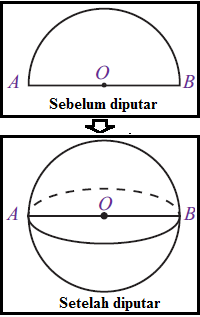
\includegraphics[width=0.5\textwidth]{figures/bola1.png}
    \caption{contoh bola}
    \label{bola1}
\end{figure}

Dalam bangun ruang, bola adalah bangun ruang tiga dimensi yang dibentuk sehingga tak terhingga lingkaran yang berjari-jari sama panjangnya dan berpusat pada satu titik yang sama. Bola merupakan bangun ruang sisi lengkung yang dibatasi oleh satu bidang lengkung.
contoh bangun ruang bola dalam kehidupan sehari-hari adalah dalam sebuah olah raga sepak bola, basket, kasti, bowling, dan sebagai nya. bola dapat menggelinding dan dapat memantul dengan sempurna, karena tidak adanya sudut pada bola. 
Bentuk bumi pun seperti bola, terlihat pada sebuah dokumentasi dari pesawat ruang angkasa, maupun dalam hal perjalan lurus, pasti akan kembali lagi ketempat kita memulai perjalanan.
Bola dapat dibentuk dari bangun setengah lingkaran yang diputar sejauh 360° pada garis tengahnya. 
Pada gambar  \ref{bola1} merupakan setengah lingkaran dengan diameter AB  tersebut dan dapat diputar satu putaran dengan diameter sebagai suatu sumbu putar maka akan tampak gambar seperti di bawahnya yang disebut bangun ruang.


Bola merupakan bangun ruang sisi lengkung (BRSL) yang terjadi dari tumpukan empat buah lingkaran \ref{sisilengkung}.
\begin{figure}[ht]
    \centering
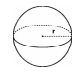
\includegraphics[width=0.25\textwidth]{figures/sisilengkung.png}
    \caption{contoh sisi lengkung}
    \label{sisilengkung}
    \end{figure} 
Keempat lingkaran ini dinamakan kulit bola. Kulit bola berada pada sisi luar bola atau mengelilingi bola \cite{nurfarikhin2010hubungan}.

Rumus bola:

a) Luas permukaan
 \begin{equation}
     L = 4 \pi r^2 \,
\end{equation}
b) Volume
\begin{equation}
     V = \frac{4}{3}\pi r^3
\end{equation}
\subsubsection{Sifat-sifat pada bola} 
a) Memiliki 1 sisi yang berbentuk bidang lengkung (selimut bola) 
b) Tidak memiliki rusuk 
c) Tidak memiliki titik sudut
 
Adapun unsur-unsur bangun ruang bola yang terdapat pada gambar \ref{unsurbola} sebagai berikut.
\begin{figure}[ht]
    \centerline{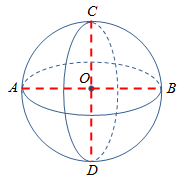
\includegraphics[width=1\textwidth]{figures/unsurbola.png}}
    \caption{contoh usur bola}
    \label{unsurbola}
    \end{figure}
1) Titik pada titik O dinamakan titik pusat bola.
2) Ruas garis pada OA disebut sebagai jari-jari pada bola. Sebutkan jari-jari pada bola lainnya.
3) Ruas garis pada CD diberi nama sebagai diameter pada bola. Jika kita amati, ruas pada garis AB tersebut merupakan diameter bola. AB dapat pula disebut sebagai tinggi bola.
4) Sisi bola merupakan kumpulan titik - titik yang mempunyai jarak yang sama terhadap titik O. Sisi tersebut dinamakan selimutatau kulit bola.
5) Ruas garis ACB dinamakan tali busur bola.
6) Ruas-ruas pada garis selimut bola yaitu ACBDA dinamakan garis pelukis bola.

\subsubsection{Konsep luas permukaan Bola}
Penentuan luas sisis (permukaan) bola dapat kita lakukan dengan sebuah percobaan archimedes, yaitu:
Sebuah bola menempati sebuah tabung yang memiliki diameter dan tinggi tabung sama tepat dengan 
yang dimiliki oleh diameter bola, maka luas bola itu sama dengan luas selimut tabung \ref{bolatabung}.
\begin{figure}[ht]
    \centerline{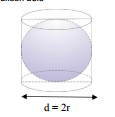
\includegraphics[width=1\textwidth]{figures/bolatabung.png}}
    \caption{sebuah bola yang terdapat dalam tabung, untuk mengukur luar permukaan tabung}
    \label{bolatabung}
    \end{figure} 
Berdasarkan gambar maka diperoleh :

Luas selimut tabung 
\begin{equation}
					L= 2 pr. T
                    = 2pr. 2r
                    = 4pr2
\end{equation}
            
\subsubsection{Konsep volume bola}
Apabila kita mengisi air ke dalam bangun bola secara penuh 
kemudian menuangkannya ke bangun ruang tabung maka air yang diperoleh adalah 2/3 bagian dari volume bangun ruang tabung tersebut. 
Dengan ketentuan bahwa kedua bangun tersebut memiliki jari-jari yang sama sehingga diperoleh:
\begin{equation}
Volume bola = 2/3 . volume tabung(silinder)
            = 2/3 . (pr2 . 2r)
\end{equation}

\subsubsection{Asal-usul rumus permukaan bola}
Jika ingin mendapatkan rumus permukaan bola, kita mulai kegiatan berikut ini untuk menguji rumus tersebut.
1. Sediakan sebuah bola berukuran sedang seperti bola sepak atau bola basket.
2. Ukurlah setiap keliling bola tersebut menggunakan benang.
3. Lilitkan benang tersebut pada permukaan setengah bola sampai penuh, seperti gambar \ref{bola2}.
\begin{figure}[ht]
    \centerline{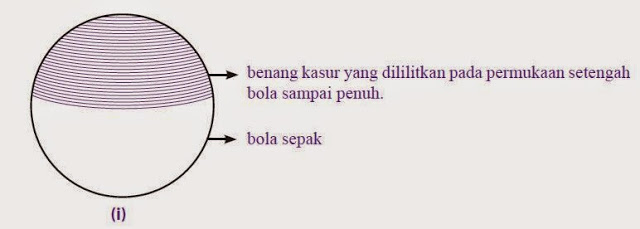
\includegraphics[width=1\textwidth]{figures/bola2.jpg}}
    \caption{gambar bola}
    \label{bola2}
    \end{figure}
4. Buatlah persegi panjang dari kertas karton dengan ukuran panjang sama dengan keliling bola dan lebar sama dengan diameter bola seperti gambar \ref{bola3}.
\begin{figure}[ht]
    \centerline{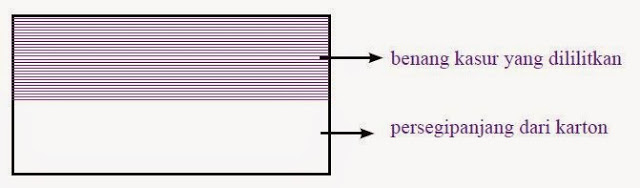
\includegraphics[width=1\textwidth]{figures/bola3.jpg}}
    \caption{beberapa kumpulan gambar yang termasuk dalam bangun ruang}
    \label{bola3}
    \end{figure}
5. Lilitkan benang yang telah digunakan untuk melilit permukaan setengah bola pada persegipanjang yang kamu buat tadi. Lilitkan sampai habis.
6. Jika kamu melakukannya dengan baik, tampak benang tersebut menutupi persegi panjang selebar jari-jari bola (r).
7. Hitunglah luas dari persegi panjang yang telah ditutupi benang tersebut. 
\begin{equation}
Luas permukaan setengah bola = luas persegi panjang
                                           = p × l
                                           = 2πr× r
                                           = 2π r2
\end{equation}

Jadi, luas permukaan bola dirumuskan sebagai berikut :
\begin{equation}
Luas permukaan bola ( L = 4πr2 )
\end{equation}
Keterangan :
L = luas permukaan bola.
r = jari-jari bola.
π = 22/7 atau 3,14

\subsubsection{Asal-usul rumus volume bola}
Cara - cara untuk mengetahui rumus volume bola, dapat dilakukan dengan cara - cara seperti berikut ini : 
1. Siapkan sebuah tempat yang berbentuk setengah bola berjari-jari r (\ref{wadah1}) dan sebuah wadah yang berbentuk kerucut berjari-jari r dan tingginya 2r (\ref{wadah2}).
2. Isikan pasir ke \ref{wadah2} sampai penuh.
3. Pindahkan pasir di dalam \ref{wadah2} ke \ref{wadah1}. Apakah yang terjadi?
\begin{figure}[ht]
    \centerline{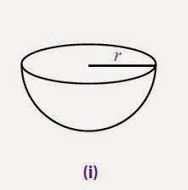
\includegraphics[width=1\textwidth]{figures/wadah1.jpg}}
    \caption{wadah dalam bola}
    \label{wadah1}
    \end{figure}
\begin{figure}[ht]
    \centerline{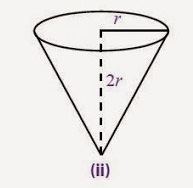
\includegraphics[width=1\textwidth]{figures/wadah2.jpg}}
    \caption{pasir dalam wadah}
    \label{wadah2}
    \end{figure}

Dari cara seperti diatas tersebut, dapat dilihat bahwasanya volume dari pasir yang dituangkan ke dalam wadah setengah bola tidak dapat berubah. Ini berarti, untuk membangun setengah bola, dan kerucut yang berjari-jari sama, dan tinggi kerucut sama dengan dua kali jari-jarinya maka:
\begin{equation}
Volume setengah bola = volume kerucut
1/2 volume bola = 1/3 πr2t
volume bola = 2/3πr2(2r)
                         = 4/3πr3
\end{equation}
Jadi, volume bola tersebut dirumuskan sebagai berikut :
\begin{equation}
Volume bola ( V = 4/3πr3 )
\end{equation}
Keterangan :
V = volume bola.
r = jari-jari bola.
π =22/7 atau 3,14.

Contoh soal :
bola memiliki jari-jari 9 cm, hitunglah volume bola tersebut ?

Jawab :
Diketahui : r = 9 cm
Ditanyakan : volume bola ?
Penyelesaian :
\begin{equation}
V   = 4/3pr3
    = 4/3/ 3 , 14 . (9)3
    = 3.052,08
\end{equation}
Jadi, volume bola tersebut 3.052,08 cm3